\documentclass[letterpaper]{article}
%Comments in Latex are made with %
%For math symbols
\usepackage{amsmath} 
%For Graphics
\usepackage{graphicx}
%Setup Page
%\usepackage{fullpage} 
\usepackage[margin=.5in]{geometry}
\usepackage{fancyhdr}
\pagestyle{fancy}
\setlength{\headheight}{14pt}

%Keep track of problems
\newcounter{problem}
\newcommand{\problem}{\refstepcounter{problem}{\vspace{2\baselineskip}\noindent\large \bfseries Problem~\arabic{problem}}.  }

%Start of document
\begin{document}
%Header
\chead{HW 1}
\lhead{Your Name, email@address.com}
\rhead{\date}
In this document I am illustrating how you might use latex to type up your homework.

%First Problem
\problem Taylor Theorem for $f(x)=e^x$ in latex:
First recall that 
%The * denotes that there will be no equation numbers
\begin{equation}
\frac{d^{i}f}{dx^i}=f^{(i)}(x)=e^x,
\end{equation}
which is a consequence of the derivative of $e^x$ being $e^x$.
%eqnarray is used for equations that span several lines
% The * indicates that there will be no equation numbers
Now from Taylor's Theorem, we have
\begin{eqnarray*}
f(x)&= &e^x,\\
&=&\sum_{i=0}^\infty\frac{x^i}{i!},\\
&=&\sum_{i=0}^n\frac{x^i}{i!}+\frac{1}{n!}\int_0^xx^{n}e^tdt,\\
&=&\sum_{i=0}^n\frac{x^i}{i!}+\frac{x^{n+1}}{(n+1)!}e^{c_x}.
\end{eqnarray*}
Let $R(x)=\frac{x^{n+1}}{(n+1)!}e^{c_x}$ (Note the size of inline equations) denote the derivative form of the error in Taylor's Theorem as applied to $e^x$.  For $x\geq 0$ we have the following bound
\begin{equation}
0\leq R(x) \leq \frac{x^{n+1}}{(n+1)!}e^{x}\leq\frac{x^{n+1}}{(n+1)!}3^{x},
\end{equation}
Where we have used three as an upper bound for $e$, and the quantity on the right can easily be computed provided we have a function for computing powers.
Plot of $e^x$ and its degree two Taylor polynomial about $x=0$.
\begin{center}
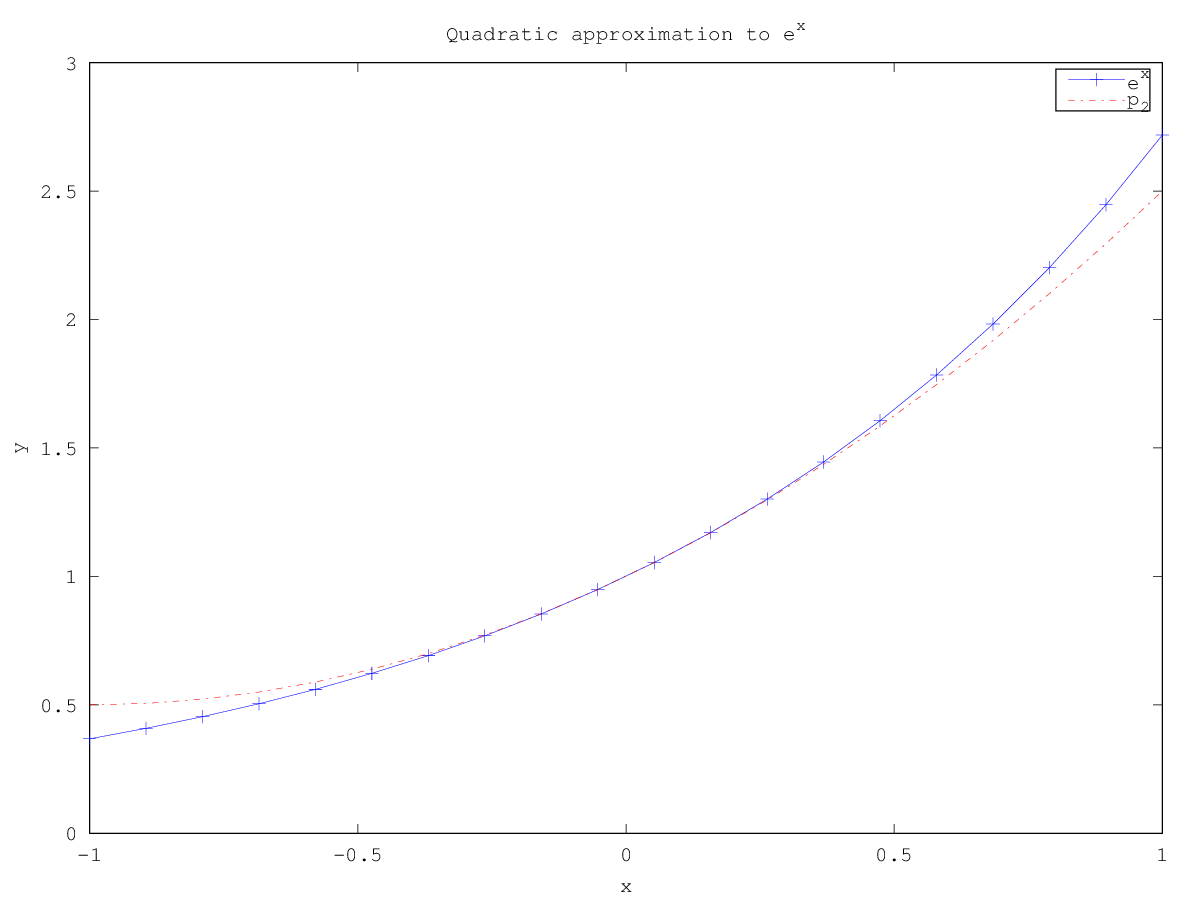
\includegraphics[scale=.45]{plot1.png}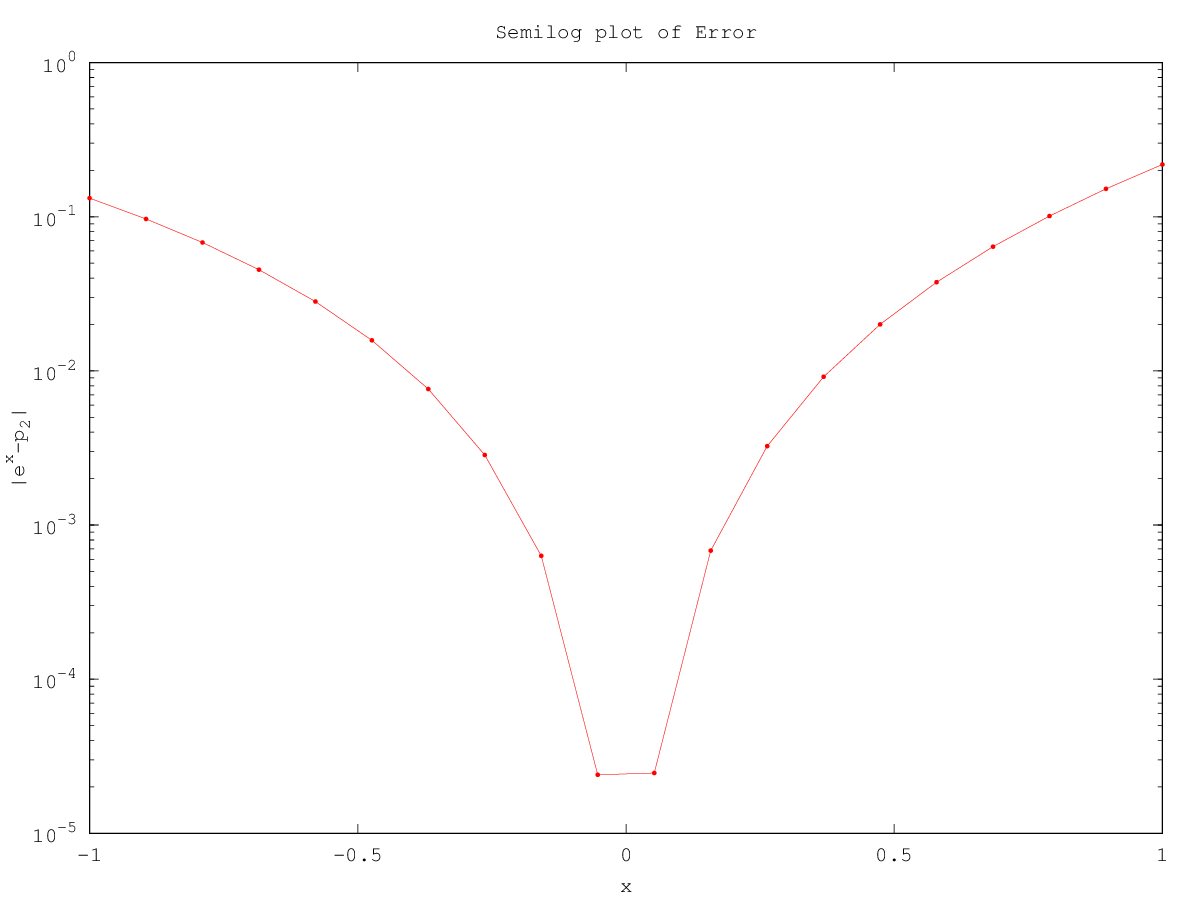
\includegraphics[scale=.45]{plot2.png}
\end{center}
Code for plot:
\begin{verbatim}
f=@(t)exp(t);
x=linspace(-1,1,20);
y=f(x);
clf
plot(x,y,'b-+');
hold on
%Taylor polynomial of degree 2 about x=0
p2=@(t)1+t+t.^2/2;
y2=p2(x);
plot(x,y2,'r-.')
%Note that the default size of a matlab figure is 8inx6in
title('Quadratic approximation to e^x')
legend('e^x','p_2')
xlabel('x')
ylabel('y')
print -dpng plot1.png
figure(2)
clf
semilogy(x,abs(y2-y),'r.-')
title('Semilog plot of Error')
xlabel('x')
ylabel('|e^x-p_2|')
print -dpng plot2.png
\end{verbatim}
%Latex has various techniques for formatting tables.  Rather than fancy tables
% I prefer well formatted printouts.  
Table for data in the figures
\begin{verbatim}
         x        e^x     p_2(x)  |e^x-p_2(x)|
-1.0000000  0.3678794  0.5000000     0.1321206
-0.8947368  0.4087151  0.5055402     0.0968250
-0.7894737  0.4540837  0.5221607     0.0680769
-0.6842105  0.5044884  0.5498615     0.0453731
-0.5789474  0.5604880  0.5886427     0.0281546
-0.4736842  0.6227039  0.6385042     0.0158003
-0.3684211  0.6918258  0.6994460     0.0076202
-0.2631579  0.7686205  0.7714681     0.0028476
-0.1578947  0.8539397  0.8545706     0.0006310
-0.0526316  0.9487295  0.9487535     0.0000240
 0.0526316  1.0540412  1.0540166     0.0000246
 0.1578947  1.1710429  1.1703601     0.0006828
 0.2631579  1.3010321  1.2977839     0.0032482
 0.3684211  1.4454505  1.4362881     0.0091624
 0.4736842  1.6058998  1.5858726     0.0200272
 0.5789474  1.7841594  1.7465374     0.0376220
 0.6842105  1.9822063  1.9182825     0.0639238
 0.7894737  2.2022370  2.1011080     0.1011290
 0.8947368  2.4466918  2.2950139     0.1516780
 1.0000000  2.7182818  2.5000000     0.2182818
\end{verbatim}
Code for generating table.
\begin{verbatim}
%Print header followed by table
fprintf('%10s %10s %10s %13s\n','x','e^x','p_2(x)','|e^x-p_2(x)|') ,for i=1:20
  fprintf('%10.7f %10.7f %10.7f %13.7f\n',x(i),y(i),y2(i), abs(y(i)-y2(i)))
end
\end{verbatim}
\problem  Much of what we do in this course generalizes to large sets of data.
For large data, it is more convenient to use of matrix notation.  A system of equations 
of the form 
\begin{equation}
\begin{array}{cccc}
a_{11}x_1&+a_{12}x_2&+a_{13}x_3&=b_1,\\
a_{21}x_1&+a_{22}x_2&+a_{23}x_3&=b_2,\\
a_{31}x_1&+a_{32}x_2&+a_{33}x_3&= b_3,
\end{array}
\end{equation}
would be written as 
\begin{equation}
Ax=b,\mbox{ where }
\end{equation}
\begin{equation}
A=\left[\begin{array}{ccc} 
a_{11}& a_{12}&a_{13}\\
a_{21}& a_{22}&a_{23}\\
a_{31}& a_{32}&a_{33}\\
\end{array}\right],\ 
x=\left(\begin{array}{c}x_1\\x_2\\x_3\end{array}\right)\mbox{ and }
b=\left(\begin{array}{c}b_1\\b_2\\b_3\end{array}\right).
\end{equation}



\end{document}